\documentclass{ximera}
%\usepackage{todonotes}

\newcommand{\todo}{}

\usepackage{tkz-euclide}
\tikzset{>=stealth} %% cool arrow head
\tikzset{shorten <>/.style={ shorten >=#1, shorten <=#1 } } %% allows shorter vectors

\usepackage{tkz-tab}  %% sign charts
\usetikzlibrary{decorations.pathreplacing} 

\usetikzlibrary{backgrounds} %% for boxes around graphs
\usetikzlibrary{shapes,positioning}  %% Clouds and stars
\usetikzlibrary{matrix} %% for matrix
\usepgfplotslibrary{polar} %% for polar plots
\usetkzobj{all}
\usepackage[makeroom]{cancel} %% for strike outs
%\usepackage{mathtools} %% for pretty underbrace % Breaks Ximera
\usepackage{multicol}

\usepackage{polynom}



\usepackage[many]{tcolorbox}  %% for titled boxes
\newtcolorbox{xbox}[1]{%
    tikznode boxed title,
    enhanced,
    arc=0mm,
    interior style={white},
    attach boxed title to top center= {yshift=-\tcboxedtitleheight/2},
    fonttitle=\bfseries,
    colbacktitle=white,coltitle=black,
    boxed title style={size=normal,colframe=white,boxrule=0pt},
    title={#1}}


\usepackage{array}
\setlength{\extrarowheight}{+.1cm}   
\newdimen\digitwidth
\settowidth\digitwidth{9}
\def\divrule#1#2{
\noalign{\moveright#1\digitwidth
\vbox{\hrule width#2\digitwidth}}}





\newcommand{\RR}{\mathbb R}
\newcommand{\R}{\mathbb R}
\newcommand{\N}{\mathbb N}
\newcommand{\Z}{\mathbb Z}

%\renewcommand{\d}{\,d\!}
\renewcommand{\d}{\mathop{}\!d}
\newcommand{\dd}[2][]{\frac{\d #1}{\d #2}}
\newcommand{\pp}[2][]{\frac{\partial #1}{\partial #2}}
\renewcommand{\l}{\ell}
\newcommand{\ddx}{\frac{d}{\d x}}
\newcommand{\ddt}{\frac{d}{\d t}}

\newcommand{\zeroOverZero}{\ensuremath{\boldsymbol{\tfrac{0}{0}}}}
\newcommand{\inftyOverInfty}{\ensuremath{\boldsymbol{\tfrac{\infty}{\infty}}}}
\newcommand{\zeroOverInfty}{\ensuremath{\boldsymbol{\tfrac{0}{\infty}}}}
\newcommand{\zeroTimesInfty}{\ensuremath{\small\boldsymbol{0\cdot \infty}}}
\newcommand{\inftyMinusInfty}{\ensuremath{\small\boldsymbol{\infty - \infty}}}
\newcommand{\oneToInfty}{\ensuremath{\boldsymbol{1^\infty}}}
\newcommand{\zeroToZero}{\ensuremath{\boldsymbol{0^0}}}
\newcommand{\inftyToZero}{\ensuremath{\boldsymbol{\infty^0}}}



\newcommand{\numOverZero}{\ensuremath{\boldsymbol{\tfrac{\#}{0}}}}
\newcommand{\dfn}{\textbf}
%\newcommand{\unit}{\,\mathrm}
\newcommand{\unit}{\mathop{}\!\mathrm}
\newcommand{\eval}[1]{\bigg[ #1 \bigg]}
\newcommand{\seq}[1]{\left( #1 \right)}
\renewcommand{\epsilon}{\varepsilon}
\renewcommand{\iff}{\Leftrightarrow}

\DeclareMathOperator{\arccot}{arccot}
\DeclareMathOperator{\arcsec}{arcsec}
\DeclareMathOperator{\arccsc}{arccsc}
\DeclareMathOperator{\si}{Si}
\DeclareMathOperator{\proj}{proj}
\DeclareMathOperator{\scal}{scal}


\newcommand{\tightoverset}[2]{% for arrow vec
  \mathop{#2}\limits^{\vbox to -.5ex{\kern-0.75ex\hbox{$#1$}\vss}}}
\newcommand{\arrowvec}[1]{\tightoverset{\scriptstyle\rightharpoonup}{#1}}
\renewcommand{\vec}{\mathbf}
\newcommand{\veci}{\vec{i}}
\newcommand{\vecj}{\vec{j}}
\newcommand{\veck}{\vec{k}}
\newcommand{\vecl}{\boldsymbol{\l}}

\newcommand{\dotp}{\bullet}
\newcommand{\cross}{\boldsymbol\times}
\newcommand{\grad}{\boldsymbol\nabla}
\newcommand{\divergence}{\grad\dotp}
\newcommand{\curl}{\grad\cross}
%\DeclareMathOperator{\divergence}{divergence}
%\DeclareMathOperator{\curl}[1]{\grad\cross #1}


\colorlet{textColor}{black} 
\colorlet{background}{white}
\colorlet{penColor}{blue!50!black} % Color of a curve in a plot
\colorlet{penColor2}{red!50!black}% Color of a curve in a plot
\colorlet{penColor3}{red!50!blue} % Color of a curve in a plot
\colorlet{penColor4}{green!50!black} % Color of a curve in a plot
\colorlet{penColor5}{orange!80!black} % Color of a curve in a plot
\colorlet{fill1}{penColor!20} % Color of fill in a plot
\colorlet{fill2}{penColor2!20} % Color of fill in a plot
\colorlet{fillp}{fill1} % Color of positive area
\colorlet{filln}{penColor2!20} % Color of negative area
\colorlet{fill3}{penColor3!20} % Fill
\colorlet{fill4}{penColor4!20} % Fill
\colorlet{fill5}{penColor5!20} % Fill
\colorlet{gridColor}{gray!50} % Color of grid in a plot

\newcommand{\surfaceColor}{violet}
\newcommand{\surfaceColorTwo}{redyellow}
\newcommand{\sliceColor}{greenyellow}




\pgfmathdeclarefunction{gauss}{2}{% gives gaussian
  \pgfmathparse{1/(#2*sqrt(2*pi))*exp(-((x-#1)^2)/(2*#2^2))}%
}


%%%%%%%%%%%%%
%% Vectors
%%%%%%%%%%%%%

%% Simple horiz vectors
\renewcommand{\vector}[1]{\left\langle #1\right\rangle}


%% %% Complex Horiz Vectors with angle brackets
%% \makeatletter
%% \renewcommand{\vector}[2][ , ]{\left\langle%
%%   \def\nextitem{\def\nextitem{#1}}%
%%   \@for \el:=#2\do{\nextitem\el}\right\rangle%
%% }
%% \makeatother

%% %% Vertical Vectors
%% \def\vector#1{\begin{bmatrix}\vecListA#1,,\end{bmatrix}}
%% \def\vecListA#1,{\if,#1,\else #1\cr \expandafter \vecListA \fi}

%%%%%%%%%%%%%
%% End of vectors
%%%%%%%%%%%%%

%\newcommand{\fullwidth}{}
%\newcommand{\normalwidth}{}



%% makes a snazzy t-chart for evaluating functions
%\newenvironment{tchart}{\rowcolors{2}{}{background!90!textColor}\array}{\endarray}

%%This is to help with formatting on future title pages.
\newenvironment{sectionOutcomes}{}{} 



%% Flowchart stuff
%\tikzstyle{startstop} = [rectangle, rounded corners, minimum width=3cm, minimum height=1cm,text centered, draw=black]
%\tikzstyle{question} = [rectangle, minimum width=3cm, minimum height=1cm, text centered, draw=black]
%\tikzstyle{decision} = [trapezium, trapezium left angle=70, trapezium right angle=110, minimum width=3cm, minimum height=1cm, text centered, draw=black]
%\tikzstyle{question} = [rectangle, rounded corners, minimum width=3cm, minimum height=1cm,text centered, draw=black]
%\tikzstyle{process} = [rectangle, minimum width=3cm, minimum height=1cm, text centered, draw=black]
%\tikzstyle{decision} = [trapezium, trapezium left angle=70, trapezium right angle=110, minimum width=3cm, minimum height=1cm, text centered, draw=black]

\author{Steven Gubkin\and Nela Lakos}
\license{Creative Commons 3.0 By-NC}
\outcome{Identify word problems as related rates problems.}
\outcome{Solve related rates word problems.}
\outcome{Translate word problems into mathematical expressions.}
\begin{document}


\begin{exercise}


A $12$ foot ladder is leaning against a wall.  At the instant that the foot of the ladder is $3$ feet away from the wall, the foot of the ladder is moving away from the wall at a rate of $5 \frac{\textrm{ft}}{\textrm{s}}$.  At what rate is the top of the ladder falling down the wall at this time?


\begin{hint}
We \textbf{introduce the variables}  $x$, the distance from  the foot of the ladder to the wall, and $y$, the distance from the of the top of the ladder to the floor. The given rate is $\frac{dx}{dt}=5$ ft/s, and the unknown rate is $\left[\frac{dy}{dt}\right]_{x=3}$. 
\end{hint}



\begin{hint}


  \begin{image}
      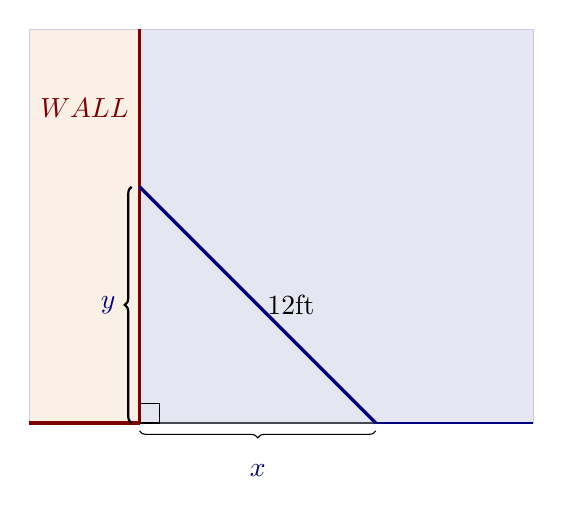
\begin{tikzpicture}
        \draw[fill1, fill=fill5!50!background] (-1.4,0) rectangle (0,5);
             \draw[fill1, fill=fill1!50!background] (0,0) rectangle (5,5);
         \coordinate (A) at (0,0);
        \coordinate (B) at (0,3);
        \coordinate (C) at (3,0);
         \coordinate (D) at (0,5);
        \tkzMarkRightAngle(C,A,B)
        \tkzDefMidPoint(A,B) \tkzGetPoint{a}
        \tkzDefMidPoint(A,C) \tkzGetPoint{b}
        \tkzDefMidPoint(B,C) \tkzGetPoint{c}
        \draw (A)--(B)--(C)--cycle;
      %  \tkzLabelPoints[right](12 ft)
          \draw[penColor2, very thick] (0,0) -- (0,5);
           \draw[penColor, thin] (3,0) -- (5,0);
           \draw[penColor, very thick] (0,3) -- (3,0);
           \draw[penColor2, very thick] (-1.4,0) -- (0,0);
     % \tkzMarkAngle[size=0.6cm,thin](B,C,A)
      \draw[decoration={brace,raise=.1cm},decorate,thick] (0,0)--(0,3);
       \draw[decoration={brace,mirror,raise=.1cm},decorate,thin] (0,0)--(3,0);
        %\tkzLabelPoints[left](a)
         
       \node [penColor2] at (-0.7,4) {$WALL$};
        \node [penColor] at (-0.4,1.5) {$y$};
        \node [right] at (c) {$12 $ft };
           \node [penColor] at (1.5,-0.6) {$x$};
             % \node [penColor] at (2.6,0.18){\small$\theta$};
      
      \end{tikzpicture}
    \end{image}
\end{hint}


\begin{hint}


	$x$ and $y$ must satisfy the relation

\[
x^2 + y^2 = 12^2
\]

by the Pythagorean theorem.
\end{hint}

\begin{hint}
	We \textbf{differentiate} with respect to time, and obtain

\[
2x(t)x'(t)+2y(t)y'(t) = 0.
\]
\end{hint}

\begin{hint}
	We \textbf{evaluate} all the quantities  at the time when $x=3$. First, we have to find the value of $y$ at that time.
\begin{align*}
	3^2 +y^2 &= 12^2\\ 
	y = \sqrt{144-9}\\
	y = \sqrt{135}.
\end{align*}
\end{hint}

\begin{hint}
	 
\begin{align*}
2(3)(5)+2\sqrt{135}\left[\frac{dy}{dt}\right]_{x=3} &=0\\
\left[\frac{dy}{dt}\right]_{x=3} = -\frac{15}{\sqrt{135}}\frac{\textrm{ft}}{\textrm{s}}.
\end{align*}

So the top of the ladder is falling at  a rate of $\frac{15}{\sqrt{135}}$ feet per second.

\end{hint}

\begin{prompt}
	The top of the ladder is falling at a rate of $\answer{\frac{15}{\sqrt{135}}}$ feet per second.
\end{prompt}

\end{exercise}

\end{document}
